\documentclass{beamer}
%\documentclass[handout]{beamer}

%\setbeamertemplate{theorems}[numbered]
\setbeamertemplate{theorems}[ams style]
\setbeamertemplate{caption}[numbered]

\usepackage{lmodern} % get rid of warnings
\usepackage{caption} % improved spacing between figure and caption

\DeclareCaptionLabelSeparator{horse}{:\quad} % change according to your needs
\captionsetup{
	labelsep = horse,
	figureposition = bottom
} 

%\usepackage[utf8]{inputenc}
\usepackage[T1]{fontenc}
\usepackage[english]{babel}

\usepackage{amsfonts}
\usepackage{amsmath}
\usepackage{amssymb}
\usepackage{amsthm}
% \usepackage[frenchstyle]{mathalpha}
% \usepackage[OMLmathsfit]{isomath}
\usepackage{graphicx}
\usepackage{color} % for ps_tex inclusions
\usepackage{fmtcount} % th, e.g. \ordinalnum{4}
\usepackage{algorithm, algorithmic} % algorithms
\usepackage{tikz}
\usetikzlibrary{bayesnet,calc,tikzmark}
\usetikzlibrary{shapes.geometric}
\tikzset{  net/.style={draw,trapezium,trapezium angle=65,shape border rotate=270} }
\tikzset{  rnn/.style={draw,rectangle} }
\usepackage{xr}
\usepackage{hyperref}
\externaldocument[notes-]{notes}
\usetheme{Madrid}
\usecolortheme{seagull}

\newcommand{\itb}{\item[$\bullet$]}
\newcommand{\dps}{\displaystyle}

\def\<{{\guillemotleft}}
\def\>{{\guillemotright}}

\def\vs1{\vspace{1mm}}
\def\v3{\vspace{3mm}}

\newcommand{\II}{\,\mbox{I\hskip -0.600em 1}}

\newcommand{\BSX}{{\boldsymbol X}}
\newcommand{\BSY}{{\boldsymbol Y}}
\newcommand{\BSZ}{{\boldsymbol Z}}

\newcommand{\bsx}{{\boldsymbol x}}
\newcommand{\bsy}{{\boldsymbol y}}
\newcommand{\bsz}{{\boldsymbol z}}

\newcommand{\bsalpha}{{\boldsymbol \alpha}}

\newcommand{\MA}{{\mathcal A}}
\newcommand{\MB}{{\mathcal B}}
\newcommand{\MC}{{\mathcal C}}
\newcommand{\MD}{{\mathcal D}}
\newcommand{\ME}{{\mathcal E}}
\newcommand{\MF}{{\mathcal F}}
\newcommand{\MG}{{\mathcal G}}
\newcommand{\MK}{{\mathcal K}}
\newcommand{\MM}{{\mathcal M}}
\newcommand{\MN}{{\mathcal N}}
\newcommand{\MO}{{\mathcal O}}
\newcommand{\MQ}{{\mathcal Q}}
\newcommand{\MS}{{\mathcal S}}
\newcommand{\MT}{{\mathcal T}}
\newcommand{\MU}{{\mathcal U}}
\newcommand{\MV}{{\mathcal V}}
\newcommand{\MX}{{\mathcal X}}

\newcommand{\TY}{{\tilde Y}}

\newcommand{\NN}{\ensuremath{\mathbb{N}}}
\newcommand{\RR}{\ensuremath{\mathbb{R}}}

\newcommand{\card}{\mbox{card}}
\newcommand{\pa}{\mbox{pa}}

\newcommand{\De}{\mbox{De}}
\newcommand{\Nd}{\mbox{Nd}}
\newcommand{\Ne}{\mbox{Ne}}

\newcommand{\indep}{\perp\!\!\!\perp}
\newcommand{\condindep}[3]{#1 \indep #2 \vert #3}
\newcommand{\condindepP}[4]{#1 \indep_{#4} #2 \vert #3}
\newcommand{\ts}[3]{#1_{#2}^{#3}}
\newcommand{\set}[1]{\{#1\}}

\newcommand{\myth}[1]{#1^{\mbox{\scriptsize{th}}}}


\newcommand{\myarray}[2]{\left(\begin{array}{#1}#2\end{array}\right)}

\title[LPC]{Learning, Probabilities, and Causality}

\subtitle{Chapter VII - Advanced Models} % (optional)

\author[Xavi]{Xavier Alameda-Pineda}
% - Use the \inst{?} command only if the authors have different
%   affiliation.

\institute{}

\date{}

\makeatother
\setbeamertemplate{footline}
{
  \leavevmode%
%   \hbox{%
%   \begin{beamercolorbox}[wd=.4\paperwidth,ht=2.25ex,dp=1ex,center]{author in head/foot}%
%     \usebeamerfont{author in head/foot}\insertshortauthor
%   \end{beamercolorbox}%
%   \begin{beamercolorbox}[wd=.6\paperwidth,ht=2.25ex,dp=1ex,center]{title in head/foot}%
    \usebeamerfont{title in head/foot}\hfill
    \insertframenumber{} / \inserttotalframenumber\hspace*{1ex}
%   \end{beamercolorbox}}%
%   \vskip0pt%
}
\makeatletter
\setbeamertemplate{navigation symbols}{}

\AtBeginSection[]{
  \begin{frame}
  \vfill
  \centering
  \begin{beamercolorbox}[sep=8pt,center,shadow=true,rounded=true]{title}
    \usebeamerfont{title}\insertsectionhead\par%
  \end{beamercolorbox}
  \vfill
  \end{frame}
}

% \newcommand{\py}{\textcolor{green}{\texttt{|py|}}}
\newcommand{\py}{\includegraphics[height=4mm]{fig/mnist/jupyter_logo.png}}

\newcommand{\bs}[1]{\boldsymbol{#1}}

%%%%%%%%%%%%%%%%%%%%%%%%%%%%%%%%%%%%%%%%%%%%%%%%%%%%%%%%%%%%%%

\begin{document}

\begin{frame}
    \titlepage
    \vspace{-1.9cm}
\end{frame}

% \begin{frame}{Outline}
%  \tableofcontents
% \end{frame}
% 
%%%%%%%%%%%%%%%%%%%%%%%%%%%%%%%%%%%%%%%%%%%%%%%%%%%%%%%%%%%%%%
\section{Dynamical VAE}
%%%%%%%%%%%%%%%%%%%%%%%%%%%%%%%%%%%%%%%%%%%%%%%%%%%%%%%%%%%%%%

%%%%%%%%%%%%%%%%%%%%%%%%%%%%%%%%%%%%%%%%%%%%%%%%%%%%%%%%%%%%%%
\begin{frame}{Let's recall the VAE}
 \only<1>{Let's try to remember altogether ;)}
\only<2>{The models ($\bs{\Theta}$ and $\bs{\Phi}$ are the parameters of the respective networks):
\begin{itemize}
\item \textbf{Gen/dec}: $p(\bs{x}|\bs{z})=\MN(\bs{x};\bs{\mu}_{\bs{\Theta}}(\bs{z}),\bs{\Sigma}_{\bs{\Theta}}(\bs{z}))$, $p(\bs{z})=\mathcal{N}(\bs{0},\bs{I})$
\item \textbf{Inf/enc}: $p(\bs{z}|\bs{x})\approx q(\bs{z}|\bs{x}) = \MN(\bs{z};\tilde{\bs{\mu}}_{\bs{\Phi}}(\bs{x}),\tilde{\bs{\Sigma}}_{\bs{\Phi}}(\bs{x}))$
\end{itemize}\vspace{3mm}

The loss (\textbf{ELBO}) needs \textbf{sampling}, $\hat{\bs{z}}_1,\ldots,\hat{\bs{z}}_R \sim q_{\bs{\Phi}}$:
\begin{align}
  \mathcal{L}_{\text{ELBO}}(\bs{\Theta},\bs{\Phi}) &= \underbrace{\frac{1}{R}\sum_{r=1}^R\log p_{\bs{\Theta}}(\bs{x}|\hat{\bs{z}}_r)}_{\text{Reconstruction}} -  \underbrace{D_{\text{KL}}\Big(q_{\bs{\Phi}}(\bs{z}|\bs{x})\Big\lVert p(\bs{z})\Big)}_{\text{Regularisation}}
\end{align}
 We use the \textbf{reparametrisation trick}: $\hat{\bs{z}}_r^{\bs{\Phi}} = \tilde{\bs{\Sigma}}_{\bs{\Phi}}^{1/2}\hat{\bs{\epsilon}}_r + \tilde{\bs{\mu}}_{\bs{\Phi}}, \hat{\bs{\epsilon}}_r\sim \MN(\bs{0},\bs{I})$\vspace{3mm}
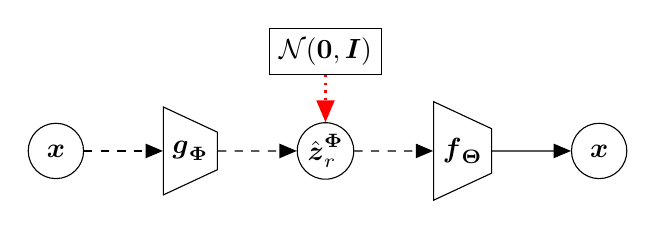
\begin{tikzpicture}[->]
   \node[latent,draw] (xi) {$\bs{x}$};
   \node[net,draw,right=of xi] (enc) {$\bs{g}_{\bs{\Phi}}$};
   \node[latent,draw,right=of enc] (z)  {$\hat{\bs{z}}_r^{\bs{\Phi}}$};
   \node[net,draw,right=of z] (dec) {$\bs{f}_{\bs{\Theta}}$};
   \node[latent,draw,right=of dec] (x) {$\bs{x}$};
   \node[draw,above=of z,yshift=-4mm] (standard) {$\MN(\bs{0},\bs{I})$};
   \edge[dashed] {xi} {enc};
   \edge[dashed] {enc} {z};
   \edge[dotted,thick,red] {standard} {z};
   \edge[dashed] {z} {dec};
   \edge{dec} {x};
\end{tikzpicture}}
\end{frame}

%%%%%%%%%%%%%%%%%%%%%%%%%%%%%%%%%%%%%%%%%%%%%%%%%%%%%%%%%%%%%%
\begin{frame}{Dynamical Variational Autoencoders (DVAE) - Motivation}
\textbf{Motivation:} Many real-world data are sequential or temporal (e.g., speech, video, time series).\\
\vs1
\textbf{Standard VAE:} Assumes i.i.d.\ data, ignores temporal dependencies.\\
\vs1
\textbf{Goal:} Model latent dynamics and temporal structure in data.\\
\vs1
\textbf{Key idea:} Introduce temporal dependencies in the latent space:
\begin{itemize}
  \item Latent variables $\bs{z}_1, \ldots, \bs{z}_T$ evolve over time.
  \item Observations $\bs{x}_1, \ldots, \bs{x}_T$ evolve over time AND depend on the sequence of latent variables $\bs{z}_{1:T}$.
\end{itemize}
\end{frame}

%%%%%%%%%%%%%%%%%%%%%%%%%%%%%%%%%%%%%%%%%%%%%%%%%%%%%%%%%%%%%%
\begin{frame}{From 1st order Markov to DVAE}
LDS (Linear Dynamical Systems) and HMM (Hidden Markov Models) are special (and simple) cases of DVAE (with an exact EM):\vspace{3mm}\\
\textbf{Generative process:}
\begin{itemize}
  \item Initial state: $\bs{z}_1 \sim p_{\bs{\Theta}}(\bs{z}_1)$
  \item Transition: $\bs{z}_t \sim p_{\bs{\Theta}}(\bs{z}_t|\bs{z}_{\only<2->{{\color{green}1:}}t-1}\only<2->{{\color{blue},\bs{x}_{1:t-1}}})$
  \item Emission: $\bs{x}_t \sim p_{\bs{\Theta}}(\bs{x}_t|\bs{z}_{\only<2->{{\color{red}1:}}t}\only<2->{{\color{brown},\bs{x}_{1:t-1}}})$
\end{itemize}\vspace{3mm}

\textbf{Graphical model:}\vspace{1mm}\\
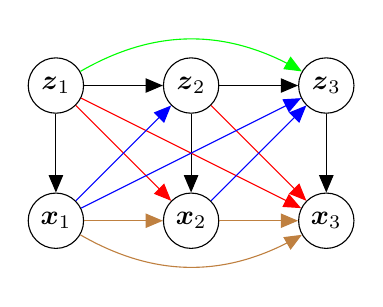
\begin{tikzpicture}[->]
  \node[latent,draw] (z1) {$\bs{z}_1$};
  \node[latent,draw,right=of z1] (z2) {$\bs{z}_2$};
  \node[latent,draw,right=of z2] (z3) {$\bs{z}_3$};
  \node[latent,draw,below=of z1] (x1) {$\bs{x}_1$};
  \node[latent,draw,below=of z2] (x2) {$\bs{x}_2$};
  \node[latent,draw,below=of z3] (x3) {$\bs{x}_3$};
  \edge {z1} {z2};
  \edge {z2} {z3};
  \edge {z1} {x1};
  \edge {z2} {x2};
  \edge {z3} {x3};
  \only<2->{
  \draw[red] (z1) -- (x2);
  \draw[red] (z1) -- (x3);
  \draw[red] (z2) -- (x3);
  \draw[blue] (x1) -- (z2);
  \draw[blue] (x1) -- (z3);
  \draw[blue] (x2) -- (z3);
  \draw[brown] (x1) -- (x2);
  \draw[brown] (x2) -- (x3);
  \path (x1) edge[->,bend right,brown] (x3);
  \path (z1) edge[->,bend left,green] (z3);
  }
\end{tikzpicture}
\end{frame}

%%%%%%%%%%%%%%%%%%%%%%%%%%%%%%%%%%%%%%%%%%%%%%%%%%%%%%%%%%%%%%
\begin{frame}{DVAE - Generative Model}
\textbf{Generative process:}
\begin{itemize}
  \item Initial state: $\bs{z}_1 \sim p_{\bs{\Theta}}(\bs{z}_1)$
  \item Transition: $\bs{z}_t \sim p_{\bs{\Theta}}(\bs{z}_t|\bs{z}_{1:t-1},\bs{x}_{1:t-1})$
  \item Emission: $\bs{x}_t \sim p_{\bs{\Theta}}(\bs{x}_t|\bs{z}_{1:t},\bs{x}_{1:t-1})$
\end{itemize}\vspace{3mm}

\textbf{Joint distribution:}
\begin{align}
p_{\bs{\Theta}}(\bs{x}_{1:T},\bs{z}_{1:T}) = p_{\bs{\Theta}}(\bs{z}_1) \prod_{t=2}^T p_{\bs{\Theta}}(\bs{z}_t|\bs{z}_{1:t-1},\bs{x}_{1:t-1}) \prod_{t=1}^T p_{\bs{\Theta}}(\bs{x}_t|\bs{z}_{1:t},\bs{x}_{1:t-1})
\end{align}
Can we rewrite the previous expression as?
\begin{align}
p_{\bs{\Theta}}(\bs{x}_{1:T},\bs{z}_{1:T}) = p_{\bs{\Theta}}(\bs{z}_{1:T}) p_{\bs{\Theta}}(\bs{x}_{1:T}|\bs{z}_{1:T})
\end{align}
\end{frame}

%%%%%%%%%%%%%%%%%%%%%%%%%%%%%%%%%%%%%%%%%%%%%%%%%%%%%%%%%%%%%%
\begin{frame}{Implementing a DVAE generative model}

\begin{columns}
\begin{column}{0.18\textwidth}
\scalebox{0.55}{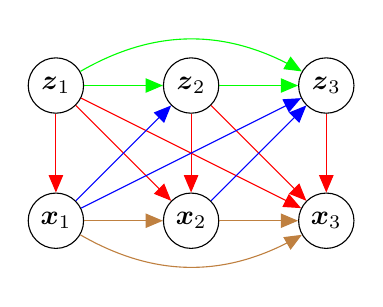
\begin{tikzpicture}[->]
  \node[latent,draw] (z1) {$\bs{z}_1$};
  \node[latent,draw,right=of z1] (z2) {$\bs{z}_2$};
  \node[latent,draw,right=of z2] (z3) {$\bs{z}_3$};
  \node[latent,draw,below=of z1] (x1) {$\bs{x}_1$};
  \node[latent,draw,below=of z2] (x2) {$\bs{x}_2$};
  \node[latent,draw,below=of z3] (x3) {$\bs{x}_3$};
  \draw[green] (z1) -- (z2);
  \draw[green] (z2) -- (z3);
  \draw[red] (z1) -- (x1);
  \draw[red] (z2) -- (x2);
  \draw[red] (z3) -- (x3);
  \draw[red] (z1) -- (x2);
  \draw[red] (z1) -- (x3);
  \draw[red] (z2) -- (x3);
  \draw[blue] (x1) -- (z2);
  \draw[blue] (x1) -- (z3);
  \draw[blue] (x2) -- (z3);
  \draw[brown] (x1) -- (x2);
  \draw[brown] (x2) -- (x3);
  \path (x1) edge[->,bend right,brown] (x3);
  \path (z1) edge[->,bend left,green] (z3);
\end{tikzpicture}}
\end{column}
\begin{column}{0.82\textwidth}
Let's take the general DVAE generative models:\vspace{-2mm}
$$ p_{\bs{\Theta}}(\bs{x}_{1:T}, \bs{z}_{1:T} ) =  \prod_{t=1}^T  p_{\bs{\Theta}_{\bs{z}}}(\bs{z}_t | {\color{blue}\bs{x}_{1:t-1}}, {\color{green}\bs{z}_{1:t-1}} ) p_{\bs{\Theta}_{\bs{x}}}(\bs{x}_t | {\color{brown}\bs{x}_{1:t-1}}, {\color{red}\bs{z}_{1:t}} ).$$
\end{column}
\end{columns}\vspace{3mm}
\pause

How to implement these distributions? (Let's do it in the blackboard)\vspace{3mm} \pause\\



The generative distributions can be implemented with an RNN:
\begin{align}
 & {\color{black}\bs{h}_{t}^{\bs{z}}} = \sigma(\bs{W}_{xh}^{\bs{z}} {\color{blue}\bs{x}_{t-1}} + \bs{W}_{zh}^{\bs{z}} {\color{green}\bs{z}_{t-1}}  + \bs{W}_{hh}^{\bs{z}} {\color{black}\bs{h}_{t-1}^{\bs{z}}} + \bs{b}_h^{\bs{z}})\\
 & p_{\bs{\Theta}_{\color{black}\bs{z}}}({\color{black}\bs{z}_t} | {\color{blue}\bs{x}_{1:t-1}}, {\color{green}\bs{z}_{1:t-1}} ) = \mathcal{N}\Big({\color{black}\bs{z}_t}; \boldsymbol{\mu}_{\bs{\Theta}_{\color{black}\bs{z}}}( {\color{black}\bs{h}_{t}^{\bs{z}}} ), \text{diag}\{ \bs{v}_{\bs{\Theta}_{\color{black}\bs{z}}}( {\color{black}\bs{h}_{t}^{\bs{z}}}) \} \Big)
\end{align}
and
\begin{align}
 & {\color{black}\bs{h}_{t}^{\bs{x}}} = \sigma(\bs{W}_{xh}^{\bs{x}} {\color{brown}\bs{x}_{t-1}} + \bs{W}_{zh}^{\bs{x}} {\color{red}\bs{z}_{t}}  + \bs{W}_{hh}^{\bs{x}} {\color{black}\bs{h}_{t-1}^{\bs{x}}} + \bs{b}_h^{\bs{x}})\\
 & p_{\bs{\Theta}_{\color{black}\bs{x}}}({\color{black}\bs{x}_t} | {\color{brown}\bs{x}_{1:t-1}}, {\color{red}\bs{z}_{1:t}} ) = \mathcal{N}\Big({\color{black}\bs{x}_t}; \boldsymbol{\mu}_{\bs{\Theta}_{\color{black}\bs{z}}}( {\color{black}\bs{h}_{t}^{\bs{x}}} ), \text{diag}\{ \bs{v}_{\bs{\Theta}_{\color{black}\bs{x}}}( {\color{black}\bs{h}_{t}^{\bs{x}}}) \} \Big)
\end{align}\pause

Can we implement with a single RNN? \pause There are \alert{many ways}, check \url{https://github.com/XiaoyuBIE1994/DVAE-speech}.
\end{frame}

%%%%%%%%%%%%%%%%%%%%%%%%%%%%%%%%%%%%%%%%%%%%%%%%%%%%%%%%%%%%%%
\begin{frame}{DVAE - Inference Model}
\textbf{Inference (encoder) network:}
\begin{itemize}
  \item Approximate posterior: $q_{\bs{\Phi}}(\bs{z}_{1:T}|\bs{x}_{1:T})$
  \item Often factorised as: $q_{\bs{\Phi}}(\bs{z}_1|\bs{x}_{1:T}) \prod_{t=2}^T q_{\bs{\Phi}}(\bs{z}_t|\bs{z}_{1:t-1},\bs{x}_{1:T})$
  \item Further simplifications are possible depending on the generative model -- found using D-separation.
  \item Implemented with RNNs, Transformers, etc.
\end{itemize}\vspace{3mm}
\end{frame}

%%%%%%%%%%%%%%%%%%%%%%%%%%%%%%%%%%%%%%%%%%%%%%%%%%%%%%%%%%%%%%
\begin{frame}{DVAE - Learning}
Recall the ELBO for VAE:
 \begin{align}
\log p(\bs{x}) &= \mathbb{E}_{q(\bs{z}|\bs{x})} \log \frac{p(\bs{x},\bs{z})}{q(\bs{z}|\bs{x})}
\end{align}

For DVAEs, the ELBO is built following the same logic. If we develop:
\begin{align}
  & \mathcal{L}(\bs{x}_{1:T}; \bs{\Phi}, \bs{\Theta}) \alert<1>{\stackrel{\only<1>{?}}{=}}
  \sum_{t=1}^T \only<1>{\mathbb{E}_{q_{\bs{\Phi}}(\bs{z}_{t} | \bs{x}_{1:T})}}\only<2->{\alert{\mathbb{E}_{q_{\bs{\Phi}}(\bs{z}_{1:t} | \bs{x}_{1:T})}} [}\underbrace{\ln p_{\bs{\Theta}_{\bs{x}}}(\bs{x}_{t} | \bs{x}_{1:t-1}, \bs{z}_{1:t})}_{\text{Reconstruction}}\only<2->{]}\\
  \nonumber& \hspace{5mm} - \sum_{t=1}^T \only<2->{\alert{\mathbb{E}_{q_{\bs{\Phi}}(\bs{z}_{1:t-1} | \bs{x}_{1:T})}} \Bigg[} \underbrace{D_{\text{KL}}\Big(q_{\bs{\Phi}}(\bs{z}_{t} | \bs{z}_{1:t-1}, \bs{x}_{1:T}) \,\Big\lVert\, p_{\bs{\Theta}_{\bs{z}}}(\bs{z}_{t} | \bs{x}_{1:t-1},  \bs{z}_{1:t-1})\Big)}_{\text{Regularization}} \only<2->{\Bigg]}  
\end{align}
\pause
\begin{itemize}
  \item The reparametrisation trick needs to be used as well.
  \item However, the sampling is \textbf{sequential} (non-parallelisable).
\end{itemize}
\end{frame}

%%%%%%%%%%%%%%%%%%%%%%%%%%%%%%%%%%%%%%%%%%%%%%%%%%%%%%%%%%%%%%
\begin{frame}{DVAE Case Study: DKF - Generative}
The Deep Kalman Filter (DKF) generative model:
\begin{equation}
  p_{\bs{\Theta}}(\bs{z}_{1:T},\bs{x}_{1:T}) = p_{\bs{\Theta}}(\bs{z}_1) \prod_{t=2}^T p_{\bs{\Theta}}(\bs{z}_t|\bs{z}_{t-1})\prod_{t=1}^T p_{\bs{\Theta}}(\bs{x}_t|\bs{z}_{t})
\end{equation}
with
\begin{align}
  &p_{\bs{\Theta}}(\bs{z}_t|\bs{z}_{t-1}) = \mathcal{N}(\bs{z}_t; \bs{\mu}_{\bs{\Theta}_z}(\bs{z}_{t-1}), \bs{\Sigma}_{\bs{\Theta}_z}(\bs{z}_{t-1})),\\
  & p_{\bs{\Theta}}(\bs{x}_t|\bs{z}_{t}) = \mathcal{N}(\bs{x}_t; \bs{\mu}_{\bs{\Theta}_x}(\bs{z}_{t}), \bs{\Sigma}_{\bs{\Theta}_x}(\bs{z}_{t})).
\end{align}
\textbf{Graphical model}: (where are the networks?)\vspace{1mm}\\
\centering
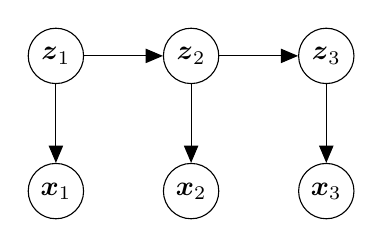
\begin{tikzpicture}[->]
  \node[latent,draw] (z1) {$\bs{z}_1$};
  \node[latent,draw,right=of z1] (z2) {$\bs{z}_2$};
  \node[latent,draw,right=of z2] (z3) {$\bs{z}_3$};
  \node[latent,draw,below=of z1] (x1) {$\bs{x}_1$};
  \node[latent,draw,below=of z2] (x2) {$\bs{x}_2$};
  \node[latent,draw,below=of z3] (x3) {$\bs{x}_3$};
  \edge {z1} {z2};
  \edge {z2} {z3};
  \edge {z1} {x1};
  \edge {z2} {x2};
  \edge {z3} {x3};
\end{tikzpicture}
\end{frame}

%%%%%%%%%%%%%%%%%%%%%%%%%%%%%%%%%%%%%%%%%%%%%%%%%%%%%%%%%%%%%%
\begin{frame}{DVAE Case Study: DKF - Inference}
\begin{center}
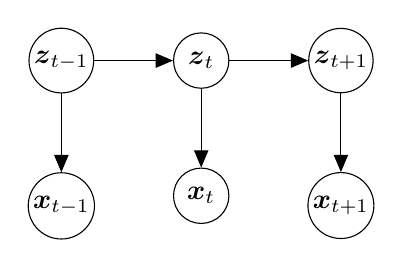
\begin{tikzpicture}[->]
  \node[latent,draw] (z1) {$\bs{z}_{t-1}$};
  \node[latent,draw,right=of z1] (z2) {$\bs{z}_{t}$};
  \node[latent,draw,right=of z2] (z3) {$\bs{z}_{t+1}$};
  \node[latent,draw,below=of z1] (x1) {$\bs{x}_{t-1}$};
  \node[latent,draw,below=of z2] (x2) {$\bs{x}_{t}$};
  \node[latent,draw,below=of z3] (x3) {$\bs{x}_{t+1}$};
  \edge {z1} {z2};
  \edge {z2} {z3};
  \edge {z1} {x1};
  \edge {z2} {x2};
  \edge {z3} {x3};
\end{tikzpicture}
\end{center}
Can we simplify the posterior distribution (using D-separation)? \only<2>{Yes:}
\begin{equation}
    q_{\bs{\Phi}}(\bs{z}_{1:T}|\bs{x}_{1:T}) = \prod_{t=1}^T q_{\bs{\Phi}}(\bs{z}_t | \bs{z}_{1:t-1} \bs{x}_{1:T}) \only<2>{= \prod_{t=1}^T q_{\bs{\Phi}}(\bs{z}_t | \bs{z}_{t-1} \bs{x}_{t:T})}
\end{equation}
We will now discuss how to implement, but let's try on the blackboard!
\end{frame}

%%%%%%%%%%%%%%%%%%%%%%%%%%%%%%%%%%%%%%%%%%%%%%%%%%%%%%%%%%%%%%
\begin{frame}{DVAE Case Study: DKF - Implementation}
The inference distribution can be implemented with a backward RNN:
\begin{align}
 & {\color{black}\bs{h}_{t}^{b}} = \sigma(\bs{W}_{xh}^{b} {\color{black}\bs{x}_{t}} + \bs{W}_{hh}^{b} {\color{black}\bs{h}_{t+1}^{b}} + \bs{b}_h^{b})\\
 & q_{\bs{\Phi}}({\color{black}\bs{z}_t} | {\color{black}\bs{x}_{t:T}}, {\color{black}\bs{z}_{t-1}} ) = \mathcal{N}\Big({\color{black}\bs{z}_t}; \boldsymbol{\mu}_{\bs{\Phi}}( {\color{black}\bs{h}_{t}^{b},\bs{z}_{t-1}} ), \text{diag}\{ \bs{v}_{\bs{\Phi}}( {\color{black}\bs{h}_{t}^{b}},\bs{z}_{t-1}) \} \Big)
\end{align}
The generative distribution can be implemented with MLP:
\begin{align}
  &p_{\bs{\Theta}}(\bs{z}_t|\bs{z}_{t-1}) = \mathcal{N}(\bs{z}_t; \bs{\mu}_{\bs{\Theta}_z}(\bs{z}_{t-1}), \bs{\Sigma}_{\bs{\Theta}_z}(\bs{z}_{t-1})),\\
  & p_{\bs{\Theta}}(\bs{x}_t|\bs{z}_{t}) = \mathcal{N}(\bs{x}_t; \bs{\mu}_{\bs{\Theta}_x}(\bs{z}_{t}), \bs{\Sigma}_{\bs{\Theta}_x}(\bs{z}_{t})).
\end{align}
\end{frame}

%%%%%%%%%%%%%%%%%%%%%%%%%%%%%%%%%%%%%%%%%%%%%%%%%%%%%%%%%%%%%%
\begin{frame}{DVAE Case Study: DKF - Loss}
Generic DVAE ELBO:
\begin{align}
  & \mathcal{L}(\bs{x}_{1:T}; \bs{\Phi}, \bs{\Theta}) =
  \sum_{t=1}^T \mathbb{E}_{q_{\bs{\Phi}}(\bs{z}_{1:t} | \bs{x}_{1:T})} [\underbrace{\ln p_{\bs{\Theta}_{\bs{x}}}(\bs{x}_{t} | \bs{x}_{1:t-1}, \bs{z}_{1:t})}_{\text{Reconstruction}}]\\
  \nonumber& \hspace{5mm} - \sum_{t=1}^T \mathbb{E}_{q_{\bs{\Phi}}(\bs{z}_{1:t-1} | \bs{x}_{1:T})} \Bigg[ \underbrace{D_{\text{KL}}\Big(q_{\bs{\Phi}}(\bs{z}_{t} | \bs{z}_{1:t-1}, \bs{x}_{1:T}) \,\Big\lVert\, p_{\bs{\Theta}_{\bs{z}}}(\bs{z}_{t} | \bs{x}_{1:t-1},  \bs{z}_{1:t-1})\Big)}_{\text{Regularization}} \Bigg]  
\end{align}
DKF ELBO (do we still need sequential sampling?):
\begin{align}
  & \mathcal{L}(\bs{x}_{1:T}; \bs{\Phi}, \bs{\Theta}) =
  \sum_{t=1}^T \mathbb{E}_{q_{\bs{\Phi}}(\bs{z}_{1:t} | \bs{x}_{1:T})} [\underbrace{\ln p_{\bs{\Theta}_{\bs{x}}}(\bs{x}_{t} | \bs{z}_{t})}_{\text{Reconstruction}}]\\
  \nonumber& \hspace{5mm} - \sum_{t=1}^T \mathbb{E}_{q_{\bs{\Phi}}(\bs{z}_{1:t-1} | \bs{x}_{1:T})} \Bigg[ \underbrace{D_{\text{KL}}\Big(q_{\bs{\Phi}}(\bs{z}_{t} | \bs{z}_{t-1}, \bs{x}_{t:T}) \,\Big\lVert\, p_{\bs{\Theta}_{\bs{z}}}(\bs{z}_{t} | \bs{z}_{t-1})\Big)}_{\text{Regularization}} \Bigg]    
\end{align}
\end{frame}

%%%%%%%%%%%%%%%%%%%%%%%%%%%%%%%%%%%%%%%%%%%%%%%%%%%%%%%%%%%%%%
\begin{frame}{DVAE Case Study: DKF - Bonus question}
HMMs, LDS, and DFKs have the \textbf{same} probabilistic dependencies:
\begin{center}
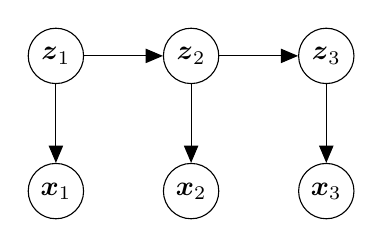
\begin{tikzpicture}[->]
  \node[latent,draw] (z1) {$\bs{z}_1$};
  \node[latent,draw,right=of z1] (z2) {$\bs{z}_2$};
  \node[latent,draw,right=of z2] (z3) {$\bs{z}_3$};
  \node[latent,draw,below=of z1] (x1) {$\bs{x}_1$};
  \node[latent,draw,below=of z2] (x2) {$\bs{x}_2$};
  \node[latent,draw,below=of z3] (x3) {$\bs{x}_3$};
  \edge {z1} {z2};
  \edge {z2} {z3};
  \edge {z1} {x1};
  \edge {z2} {x2};
  \edge {z3} {x3};
\end{tikzpicture}
\end{center}
Why do we use an EM for HMM and LDS, but SGD for DKF?\pause \vspace{3mm}\\Let us recall the formula at the core of the EM and ELBO formulations:
 \begin{align}
\log p(\bs{x}) &= \mathbb{E}_{q(\bs{z}|\bs{x})}\Big\{\log \frac{p(\bs{x},\bs{z})}{q(\bs{z}|\bs{x})}\Big\} + {\color{blue} D_{\text{KL}}\Big(q(\bs{z}|\bs{x})\Big\lVert p(\bs{z}|\bs{x})\Big)}
\end{align}
($\bs{x}=\bs{x}_{1:T}$ and $\bs{z}=\bs{z}_{1:T}$)
\end{frame}

%%%%%%%%%%%%%%%%%%%%%%%%%%%%%%%%%%%%%%%%%%%%%%%%%%%%%%%%%%%%%%
\begin{frame}{DVAE Summary}
\begin{itemize}
  \item DVAE are an extension of VAE to sequential/temporal data.
  \item They model latent dynamics and temporal dependencies in data.
  \item The generative model introduces temporal dependencies in the latent space and/or in the observation spaces.
  \item The inference model approximates the posterior over latent sequences (with the temporal dependencies associated to the generative model).
  \item Training maximises the ELBO using the reparametrisation trick and sequential sampling.
  \item Many models exist (DKF, VRNN, SRNN, etc.) and can be implemented in many ways (RNNs, Transformers, etc.).
\end{itemize}
\end{frame}

%%%%%%%%%%%%%%%%%%%%%%%%%%%%%%%%%%%%%%%%%%%%%%%%%%%%%%%%%%%%%%
\section{Diffusion Models}
\begin{frame}{From Noise to Data: The Big Idea}
   Diffusion models: gradually add noise to data (\emph{forward}) and learn to reverse the process (\emph{backward}), transforming noise into data.
   \begin{center}
    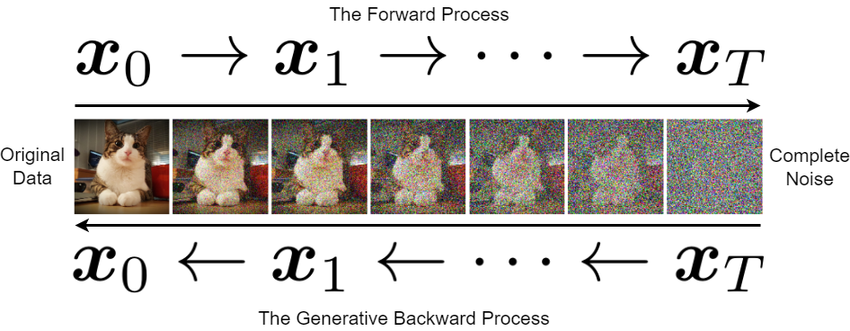
\includegraphics[width=\textwidth]{fig/diffusion_intro.png}
   \end{center}
\end{frame}

%%%%%%%%%%%%%%%%%%%%%%%%%%%%%%%%%%%%%%%%%%%%%%%%%%%%%%%%%%%%%%
\begin{frame}{DDPM: Denoising Diffusion Probabilistic Models}
 The forward process:   
  \begin{itemize}
        \item Start with data \(\bs{x}_0\); gradually add Gaussian noise in \(T\) steps:
            \[
                q(\bs{x}_t | \bs{x}_{t-1}) = \mathcal{N}(\bs{x}_t; \sqrt{1-\beta_t}\bs{x}_{t-1}, \beta_t \bs{I})
            \]
        \item At \(t = T\), \(\bs{x}_T \sim \mathcal{N}(0, \bs{I})\), nearly pure noise.
    \end{itemize}\vspace{6mm}

The Reverse Process:
    \begin{itemize}
        \item Learn \(p_{\bs{\Theta}}(\bs{x}_{t-1} | \bs{x}_t)\) to denoise:
            \[
                p_{\bs{\Theta}}(\bs{x}_{t-1} | \bs{x}_t) = \mathcal{N}(\bs{x}_{t-1}; \mu_{\bs{\Theta}}(\bs{x}_t, t), \Sigma_{\bs{\Theta}}(\bs{x}_t, t))
            \]
        \item Start with noise, step-by-step denoise to sample new data.
    \end{itemize}
\end{frame}

\begin{frame}{Markov Chains and Gaussian Transitions}
    \begin{itemize}
        \item Both forward and reverse processes are Markovian.
        \item Transition probabilities are Gaussian, enabling tractable computation.
        \item The full process: \(q(\bs{x}_{1:T} | \bs{x}_0) = \prod_{t=1}^T q(\bs{x}_t | \bs{x}_{t-1})\).
    \end{itemize}
    \textcolor{red}{Talk about latent variables. Talk about the full forward and backward processes.}
\end{frame}

\begin{frame}{Evidence Lower Bound Objective}
Rationale: $\bs{x}_0$ is the observed data, $\bs{x}_{1:T}$ are latent variables. We can compute the ELBO as usual:
\begin{equation}
  \log p_{\bs{\Theta}}(\bs{x}_0) \geq \mathbb{E}_{q(\bs{x}_{1:T}|\bs{x}_0)} \Bigg[\log \frac{p_{\bs{\Theta}}(\bs{x}_{0:T})}{q(\bs{x}_{1:T}|\bs{x}_0)}\Bigg] = \mathcal{L}
\end{equation}
and further rewrite it as:
\begin{align}
  \mathcal{L} &= D_{\text{KL}}(q(\bs{x}_T | \bs{x}_0) \| p(\bs{x}_T)) - \log p_{\bs{\Theta}}(\bs{x}_0 | \bs{x}_1) \\
  &+ \sum_{t>1} D_{\text{KL}}(q(\bs{x}_{t-1} | \bs{x}_t, \bs{x}_0) \| p_{\bs{\Theta}}(\bs{x}_{t-1} | \bs{x}_t)) 
\end{align}  
    \textcolor{red}{Verify the equation above. Include the forward-backward image. Recall the Gaussianity?}

\end{frame}

\begin{frame}{Architectures: U-Net and Beyond}
    \begin{itemize}
        \item Popular choice: U-Net with time embedding input.
        \item Conditional variants: class-conditional, text-conditional (DALL-E 2).
    \end{itemize}
\end{frame}

\section{Connecting to SDEs}
\begin{frame}{Discrete to Continuous-Time Limit}
    \begin{itemize}
        \item As the number of steps \(T \to \infty\), the process approaches a continuous diffusion:
        \item Forward SDE:
            \[
                d\bs{x} = f(\bs{x}, t)dt + g(t) d\bs{w}
            \]
            where \(d\bs{w}\) is a Wiener process.
    \end{itemize}
\end{frame}

\begin{frame}{Variance Preserving and Exploding SDEs}
    \begin{itemize}
        \item Different SDEs suit different tasks:
        \begin{itemize}
            \item Variance Preserving (VP): interpolates between data and noise.
            \item Variance Exploding (VE): rapidly adds noise.
        \end{itemize}
        \item Choice affects architecture and sampling.
    \end{itemize}
\end{frame}

\begin{frame}{Backward SDE and Denoising}
    \begin{itemize}
        \item Sample generation corresponds to solving a backward SDE.
            \[
                d\bs{x} = [f(\bs{x}, t) - g(t)^2 \nabla_{\bs{x}} \log p_t(\bs{x})]dt + g(t)d\bar{\bs{w}}
            \]
        \item The score function \(\nabla_{\bs{x}} \log p_t(\bs{x})\) plays a key role.
    \end{itemize}
\end{frame}

\begin{frame}{Score Functions and Training}
    \begin{itemize}
        \item Train a neural network to estimate the score function at various noise levels.
        \item Minimize denoising score matching loss over all times.
    \end{itemize}
\end{frame}

\begin{frame}{ODE Sampling}
    \begin{itemize}
        \item Sampling can use SDE or corresponding ODE:
            \[
                d\bs{x} = [f(\bs{x}, t) - 0.5g(t)^2 \nabla_{\bs{x}}\log p_t(\bs{x})]dt
            \]
        \item ODE sampling can yield improved, faster results.
    \end{itemize}
\end{frame}

\section{Score-Based Diffusion Models}
\begin{frame}{Score-Based Diffusion: Links}
    \begin{itemize}
        \item Score-based models directly learn \(\nabla_{\bs{x}} \log p_t(\bs{x})\).
        \item Unified view with diffusion: both approaches sample by reversing a stochastic/noisy process.
    \end{itemize}
\end{frame}

\begin{frame}{Sampling Algorithms and Extensions}
    \begin{itemize}
        \item Ancestral sampling, DDIM (Denoising Diffusion Implicit Models), other ODE/SDE solvers.
        \item Improvements in speed, flexibility, and sample quality.
    \end{itemize}
\end{frame}

\begin{frame}{Limitations and Trade-Offs}
    \begin{itemize}
        \item Pros: great sample quality, training stability, flexible architectures.
        \item Cons: slow sampling, computational cost, memory.
        \item Ongoing research: faster sampling, better priors, application domains.
    \end{itemize}
\end{frame}

\section{Summary and Further Study}
\begin{frame}{Recap and Resources}
    \begin{itemize}
        \item Key takeaways: diffusion as generative modeling via noise and denoising.
        \item SDEs connect discrete and continuous perspectives.
        \item Score-based modeling as a core unifying idea.
        \item For more, see recent surveys, open-source repos, and benchmarks.
    \end{itemize}
\end{frame}

%%%%%%%%%%%%%%%%%%%%%%%%%%%%%%%%%%%%%%%%%%%%%%%%%%%%%%%%%%%%%%
\begin{frame}{Score-based Models - Motivation}
\textbf{Motivation:} Model complex data distributions without explicit likelihoods.\\
\vs1
\textbf{Key idea:} Learn the \textbf{score function} (gradient of log-density):
\begin{equation}
  \bs{s}_{\bs{\Theta}}(\bs{x}) \approx \nabla_{\bs{x}} \log p(\bs{x})
\end{equation}
\vs1
\textbf{Applications:} Generative modeling, denoising, sampling.
\vs1
\textbf{Challenge:} $p(\bs{x})$ is unknown, but we can estimate its score from data.
\end{frame}

%%%%%%%%%%%%%%%%%%%%%%%%%%%%%%%%%%%%%%%%%%%%%%%%%%%%%%%%%%%%%%
\begin{frame}{Diffusion Models - Overview}
\textbf{Diffusion models:} Generative models based on gradual noise injection and denoising.\\
\vs1
\textbf{Forward process:} Add noise to data in $T$ steps:
\begin{equation}
  q(\bs{x}_t|\bs{x}_{t-1}) = \mathcal{N}(\bs{x}_t; \sqrt{1-\beta_t}\bs{x}_{t-1}, \beta_t \bs{I})
\end{equation}
\vs1
\textbf{Reverse process:} Learn to denoise:
\begin{equation}
  p_{\bs{\Theta}}(\bs{x}_{t-1}|\bs{x}_t)
\end{equation}
\vs1
\textbf{Sampling:} Start from noise, iteratively denoise to generate data.
\end{frame}

%%%%%%%%%%%%%%%%%%%%%%%%%%%%%%%%%%%%%%%%%%%%%%%%%%%%%%%%%%%%%%
\begin{frame}{Diffusion Models - Score-based Perspective}
\textbf{Connection to score-based models:}
\begin{itemize}
  \item The reverse process requires the score $\nabla_{\bs{x}_t} \log p(\bs{x}_t)$.
  \item Train a neural network to approximate the score at each noise level.
\end{itemize}
\vs1
\textbf{Training objective:} Denoising score matching:
\begin{equation}
  \mathbb{E}_{q(\bs{x}_0, \bs{x}_t)} \left[ \lambda_t \left\| \bs{s}_{\bs{\Theta}}(\bs{x}_t, t) - \nabla_{\bs{x}_t} \log q(\bs{x}_t|\bs{x}_0) \right\|^2 \right]
\end{equation}
\vs1
\textbf{Result:} Enables high-quality sample generation.
\end{frame}

%%%%%%%%%%%%%%%%%%%%%%%%%%%%%%%%%%%%%%%%%%%%%%%%%%%%%%%%%%%%%%
\begin{frame}{Flow-Matching Models}
\textbf{Motivation:} Learn continuous-time generative models via ODEs.\\
\vs1
\textbf{Key idea:} Model a flow that transforms noise into data:
\begin{equation}
  \frac{d\bs{x}(t)}{dt} = \bs{v}_{\bs{\Theta}}(\bs{x}(t), t)
\end{equation}
\vs1
\textbf{Flow-matching:} Train $\bs{v}_{\bs{\Theta}}$ so that the flow matches the data distribution at $t=1$ and noise at $t=0$.
\vs1
\textbf{Relation:} Generalises both diffusion and normalizing flow models.
\end{frame}

\end{document}


